\documentclass[11pt,compress,t,notes=noshow, aspectratio=169, xcolor=table]{beamer}

\usepackage{../../style/lmu-lecture}
% Defines macros and environments
\input{../../style/common.tex}
\usepackage{graphicx}
\usepackage{url}
\usepackage{amsmath}
\usepackage{amssymb}
\usepackage[utf8]{inputenc}
\usepackage[T1]{fontenc}
\usepackage{hyperref}
\usepackage{verbatim}

\usepackage{listings}

% \lstset{
%   basicstyle=\ttfamily\small,
%   columns=fullflexible,
%   keepspaces=true,
% }

\lstset{
language=R,
basicstyle=\scriptsize\ttfamily,
commentstyle=\ttfamily\color{gray},
backgroundcolor=\color{white},
%backgroundcolor=\color{light-gray}
showspaces=false,
showstringspaces=false,
showtabs=false,
frame=single,
%tabsize=3,
xleftmargin=1cm,
columns=fullflexible,
keepspaces=true,
captionpos=b,
breaklines=false,
breakatwhitespace=false,
title=\lstname,
escapeinside={},
keywordstyle={},
morekeywords={}, 
belowskip = -1.2 \baselineskip,
}
%\verb|basicstyle=\ttfamily, columns=fullflexible, keepspaces=true|


\title{Applied Machine Learning}
% \author{LMU}
%\institute{\href{https://compstat-lmu.github.io/lecture_iml/}{compstat-lmu.github.io/lecture\_iml}}
\date{}

\begin{document}

\newcommand{\titlefigure}{figure/empty}
\newcommand{\learninggoals}{
\item OpenML in R
\item batchtools}

\lecturechapter{Applied Performance Evaluation}
\lecture{Applied Machine Learning}


% %\section{Efficiency: Parallelization}
% \begin{frame}[fragile]{Efficiency: Parallelization}
%   \begin{itemize}
%     \item Parallelization minimizes effective computation time by distributing CPU time to many cores.
%     \item Speedups are theoretically linear to the number of independently run processes.
%     \item Debugging parallel code is especially hard.
%     \item Coding discipline is even more important to minimize errors and frustration.
%   \end{itemize}
% \end{frame}

% %\section{Easily Parallelizable Tasks}
% \begin{frame}[fragile]{What can be easily parallelized?}
%   \begin{itemize}
%     \item Independent replications
%     \item Resampling, cross-validation
%     \item Model averaging
%     \item Parameter variations in simulations \ldots
%     \item "Single program, multiple data"
%     \item Everything expressible as a loop of independent iterations (if you can write it with \texttt{(l|m|)apply}, you are fine)
%   \end{itemize}
%   \textbf{Many statistical problems are "embarrassingly parallel"}
% \end{frame}

% %\section{Performance Improvement}
% \begin{frame}[fragile]{Ideal performance improvement}
%   \begin{itemize}
%     \item p processors should be p times faster than one processor.
%     \item Note: This is rarely possible in practice.
%     \item For more theory, look up Amdahl's law and Gustafson's law.
%   \end{itemize}
%   \begin{table}
%     \centering
%     \begin{tabular}{|c|c|}
%       \hline
%       Single processor & 30 Processors \\
%       \hline
%       1 minute & 2 seconds \\
%       1 hour & 2 minutes \\
%       1 day & 1 hour \\
%       1 month & 1 day \\
%       1 year & 2 weeks \\
%       \hline
%     \end{tabular}
%   \end{table}
% \end{frame}

% %\section{Programming Requirements}
% \begin{frame}[fragile]{Ideal Programming Requirements}
%   \begin{itemize}
%     \item Minimal effort for simple problems
%     \item Use existing high-level (i.e., R) code
%     \item Ability to test code in a sequential setting
%     \item Debugging parallel problems possible
%     \item Seeding / Reproducibility (with different CPU settings)
%     \item Scale up to larger systems with minimal effort
%   \end{itemize}
%   \textit{As often: Cannot have your cake and eat it, too...}
% \end{frame}

% %\section{Batch Computing}
% \begin{frame}[fragile]{Naive batch computing}
%   Computing on multicore machines (non-cluster):
%   \begin{itemize}
%     \item Write standalone script(s) that run your jobs and save results at the end.
%     \item Parameters must be hard-coded or retrieved through the command line.
%     \item Login on a machine per SSH.
%     \item Start job(s) with \texttt{R CMD BATCH myscript1.R}, combine this with nohup, screen, or tmux.
%     \item Start remaining jobs when resources get available (argh...).
%     \item Check manually for completion / errors (argh again...).
%     \item Write a script to collect results.
%   \end{itemize}
%   No automation, no resource management or fair share, neither easily extensible nor scalable.
% \end{frame}

% %\section{HPC Clusters}
% \begin{frame}[fragile]{High Performance Computing (HPC) clusters}
%   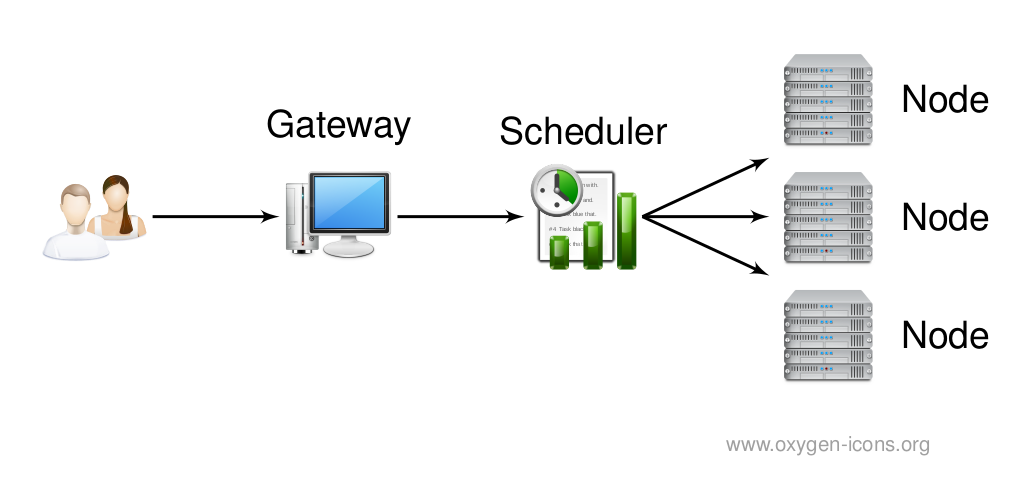
\includegraphics{figure/hpc.png}
%   \begin{itemize}
%     \item User logs into the gateway server (master or head node).
%     \item Network of multiple nodes, managed by scheduler.
%     \item Scheduler orchestrates computation and organizes queues to fairly distribute computation times among users.
%     \item Nodes usually share a file system.
%   \end{itemize}
% \end{frame}

% %\section{Batch System Workflow}
% \begin{frame}[fragile]{Manual working on a batch system}
%   You have to specify:
%   \begin{itemize}
%     \item Resource specifications (number CPUs, number of tasks, expected runtime, and memory)
%     \item Which cluster/partition to use
%     \item Command to execute (e.g., \texttt{R CMD BATCH <myscript.R>})
%   \end{itemize}
%   You have to manually:
%   \begin{itemize}
%     \item Pass specs to CLI tools, either directly as arguments or encoded in a shell script
%     \item Check the status of jobs via CLI tools (e.g., \texttt{squeue})
%     \item Write a script to collect results
%   \end{itemize}
% \end{frame}

% \begin{frame}[fragile]{Usual workflow on a batch system}
%   \begin{itemize}
%     \item Unroll your \texttt{R} loop(s) so that your script computes a single iteration.
%     \item Write a script that writes \texttt{R} scripts for each iteration setting the iteration counter(s) at the beginning.
%     \item Write a script that writes job description files for each \texttt{R} script.
%     \item Write a script that submits your job description files.
%     \item Crawl through file system checking for the existence of results or log files.
%     \item Write a script that combines your scattered result files.
%   \end{itemize}
% \end{frame}

% \begin{frame}[fragile]{Handling Issues in Batch Systems}
%   \begin{itemize}
%     \item Found a bug in your code? Write a script that kills all running jobs, fix the bug, submit everything again.
%     \item Some jobs have hit the wall time? Write a script that finds out which jobs you need to resubmit with weaker constraints.
%     \item Want to try your model on another data set or using other parameters? Eventually start from scratch, it might get ugly.
%   \end{itemize}
% \end{frame}

% %\section{Conclusions}
% \begin{frame}[fragile]{Conclusions and further remarks}
%   \begin{itemize}
%     \item Clusters are pretty fast!
%     \item Many statistical tasks are embarrassingly parallel
%   \end{itemize}
%   \textbf{But:}
%   \begin{itemize}
%     \item Job description files needed
%     \item We cannot control when jobs are started.
%     \item Jobs cannot really communicate, except by writing stuff on disk (or we have to allocate multiple cores and use something like MPI).
%     \item Requesting many nodes at once increases time spent in queue.
%     \item Auxiliary scripts to create files and submit jobs necessary.
%     \item Functions to collect results can get complicated and lengthy.
%     \item If some jobs fail (e.g., singularities), debugging is awful.
%   \end{itemize}
% \end{frame}

% \begin{frame}[fragile]{OpenML in R}
%   \begin{itemize}
%     \item \texttt{list_oml_}
%   \end{itemize}
% \end{frame}


\begin{frame}[fragile]
\frametitle{What is mlr3oml?}

% \begin{itemize}
%   \item Benchmark experiments require high-quality datasets and tasks for meaningful conclusions.
%   \item \textbf{OpenML}: An open-source platform for sharing machine learning research data, algorithms, and results.
%   \item Ensures data is \textbf{FAIR} (Findable, Accessible, Interoperable, Reusable).
% \end{itemize}

\begin{itemize}
  \item Benchmark experiments require high-quality data for meaningful conclusions.
  \item \textbf{OpenML.org}: Open-source platform for sharing entities of ML experiments.
  \item \texttt{mlr3oml} is an R package providing an interface to OpenML (via  REST API).\\
  $\Rightarrow$ Query, download, and publish data, tasks, and task collections.\\
  $\Rightarrow$ Experiment results of others can also be queried and downloaded.
\end{itemize}

\end{frame}

\begin{frame}[fragile]
\frametitle{Listing Data}
Example of filtering datasets by properties:
\begin{lstlisting}[language=R]
library(mlr3oml)
odatasets = list_oml_data(
  number_features = c(10, 20),
  number_instances = c(45000, 50000),
  number_classes = 2
)
odatasets[1:5, c(1,2,9)]
#   data_id                        name NumberOfFeatures
#     <int>                      <char>            <int>
#1:     179                       adult               15
#2:    1461              bank-marketing               17
#3:    1590                       adult               15
#4:   43898                       adult               15
#5:   44234 Bank_marketing_data_set_UCI               17
\end{lstlisting}
\end{frame}

\begin{frame}[fragile]
\frametitle{Downloading Data}
\begin{itemize}
  \item Download metadata with \texttt{odt(id = 1590)} or \texttt{OMLData\$new(id = 1590)}.
  \item Query metadata (number of rows, columns, etc.) without loading the entire data:
\end{itemize}
\begin{lstlisting}[language=R]
odata = odt(id = 1590)
class(odata)
#[1] "OMLData"   "OMLObject" "R6"   
odata$nrow
#[1] 48842
odata$ncol
#[1] 15
\end{lstlisting}

\begin{itemize}
  \item Download and store data by accessing the \texttt{\$data} field:
\end{itemize}
\begin{lstlisting}[language=R]
odata$data[1:5, 1:5]
#     age workclass fnlwgt    education education.num
#   <int>    <fctr>  <int>       <fctr>         <int>
#1:    25   Private 226802         11th             7
#2:    38   Private  89814      HS-grad             9
#3:    28 Local-gov 336951   Assoc-acdm            12
#4:    44   Private 160323 Some-college            10
#5:    18      <NA> 103497 Some-college            10
\end{lstlisting}
\end{frame}

\begin{frame}[fragile]
\frametitle{Convert Data to mlr3 Tasks}
\begin{itemize}
  \item \texttt{mlr3oml} Cache: 
  \begin{itemize}
      \item Data is cached in memory after first access.
      \item Option to cache permanently by setting\\ \texttt{options(mlr3oml.cache = tempfile())}.
  \end{itemize} 
  \item Convert data to \texttt{mlr3} tasks for seamless integration:
\end{itemize}
\begin{lstlisting}[language=R]
library(mlr3)
tsk_adult = as_task_classif(odata$data, target = "class")
tsk_adult
#<TaskClassif:odata$data> (48842 x 15)
#* Target: class
#* Properties: twoclass
#* Features (14):
#  - fct (8): education, marital.status, native.country, occupation, race, 
#    relationship, sex, workclass
#  - int (6): age, capital.gain, capital.loss, education.num, fnlwgt, 
#    hours.per.week
\end{lstlisting}
\end{frame}

\begin{frame}[fragile]
\frametitle{Listing Tasks}
\begin{itemize}
  \item OpenML tasks specify target variable, train-test splits, etc.
  \item Example of filtering tasks:
\end{itemize}
\begin{lstlisting}[language=R]
adult_tasks = list_oml_tasks(data_id = 1590)
adult_tasks[task_type == "Supervised Classification", ]
#   task_id                 task_type data_id
#     <int>                    <char>   <int>
#1:    7592 Supervised Classification    1590
#2:   14947 Supervised Classification    1590
#3:  126025 Supervised Classification    1590
#4:  146154 Supervised Classification    1590
#5:  146598 Supervised Classification    1590
#6:  168878 Supervised Classification    1590
#7:  233099 Supervised Classification    1590
#8:  359983 Supervised Classification    1590
#9:  361515 Supervised Classification    1590
\end{lstlisting}
\end{frame}

\begin{frame}[fragile]
\frametitle{Downloading Tasks}
\begin{itemize}
  \item Load task with ID 359983 and examine data and splits:
\end{itemize}
\begin{lstlisting}[language=R]
otask = otsk(id = 359983)
otask$data
otask$task_splits
\end{lstlisting}
\end{frame}

\begin{frame}[fragile]
\frametitle{Task Collections and Benchmark Suites}
\begin{itemize}
  \item Bundle tasks for benchmark suites, e.g., CC-18 benchmark suite with ID 99:
\end{itemize}
\begin{lstlisting}[language=R]
otask_collection = ocl(id = 99)
otask_collection$task_ids[1:5]
\end{lstlisting}
\begin{itemize}
  \item Define tasks and resamplings from task collection:
\end{itemize}
\begin{lstlisting}[language=R]
tasks = as_tasks(otask_collection)
resamplings = as_resamplings(otask_collection)
\end{lstlisting}
\end{frame}

\begin{frame}[fragile]
\frametitle{Filtering and Benchmarking}
\begin{itemize}
  \item Example: Binary classification tasks from CC-18 collection:
\end{itemize}
\begin{lstlisting}[language=R]
binary_cc18 = list_oml_tasks(
  limit = 6,
  task_id = otask_collection$task_ids,
  number_classes = 2
)
otasks = lapply(binary_cc18$task_id, otsk)
tasks = as_tasks(otasks)
resamplings = as_resamplings(otasks)
\end{lstlisting}
\end{frame}

\begin{frame}[fragile]
\frametitle{Benchmarking Setup}
\begin{itemize}
  \item Use \texttt{benchmark\_grid()} to set up large experiments:
\end{itemize}
\begin{lstlisting}[language=R]
large_design = benchmark_grid(tasks, learners, resamplings, paired = TRUE)
large_design[1:6]
\end{lstlisting}
\end{frame}

\begin{frame}[fragile]
\frametitle{Summary}
\begin{itemize}
  \item \texttt{mlr3oml} provides robust tools for accessing and utilizing OpenML datasets and tasks.
  \item Facilitates large-scale benchmarking and reproducible research.
\end{itemize}
\end{frame}

\begin{frame}[fragile]{Efficiency and Parallelization}
  \begin{itemize}
    \item \textbf{Goal}: Minimize computation time by distributing tasks across multiple CPU cores.
    \item \textbf{Parallelizable Tasks}: Independent replications, resampling, model averaging, parameter variations, etc.
    \item \textbf{Challenges}: Debugging and maintaining parallel code require strict coding discipline.
    \item \textbf{Performance}: Ideal speedup is linear to the number of processes, but often limited by overhead and dependencies (Amdahl's Law, Gustafson's Law).
  \end{itemize}
\end{frame}

\begin{frame}[fragile]{Programming and Batch Computing}
  \begin{itemize}
    \item \textbf{Requirements}: Minimal effort for simple problems, use existing high-level code (R), test sequentially, debug parallel code, reproducibility, scalability.
    \item \textbf{Naive Batch Computing}: Write standalone scripts, SSH login, manually check jobs, gather results.
    \item \textbf{Limitations}: No automation, no resource management, not scalable.
  \end{itemize}
\end{frame}

\begin{frame}[fragile]{HPC Clusters and Workflow}
  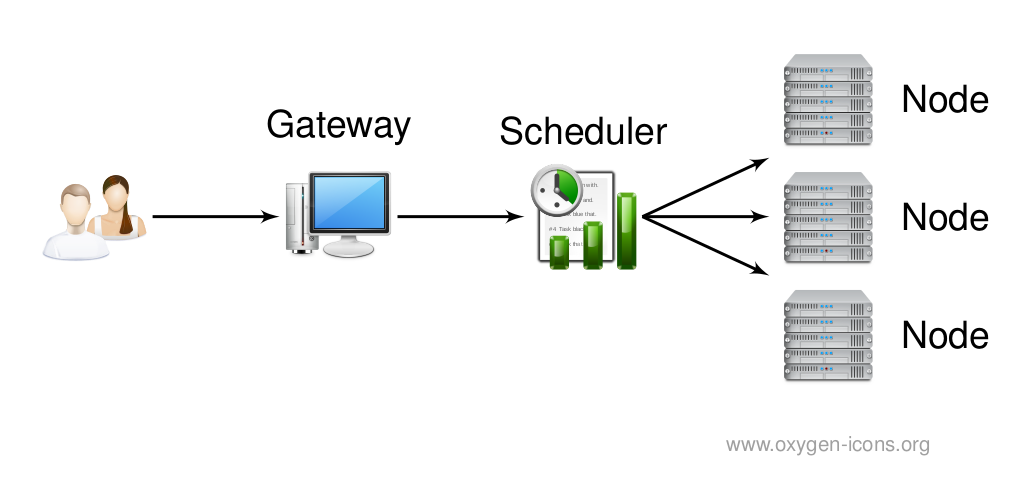
\includegraphics[width=0.6\textwidth]{figure/hpc.png}
  \begin{itemize}
    \item \textbf{HPC Clusters}: Network of nodes managed by a scheduler, shared file system.
    \item \textbf{Workflow}: Specify resources, create job description files, submit jobs, monitor and collect results.
    \item \textbf{Issues}: Handle bugs, timeouts, and parameter changes.
  \end{itemize}
\end{frame}

\begin{frame}[fragile]{Conclusions and Further Remarks}
  \begin{itemize}
    \item \textbf{Advantages}: Significant speedups, efficient parallel task handling.
    \item \textbf{Challenges}: Job description files, start time control, inter-job communication, queue times, auxiliary scripts, result collection complexity, debugging issues.
    \item \textit{Final Note}: Clusters are powerful but require careful management and coding discipline.
  \end{itemize}
\end{frame}

\begin{frame}[fragile]{batchtools}
  \begin{itemize}
    \item Basic infrastructure to communicate with a high performance cluster
    \item Tailored around Map-Reduce paradigm
    \item Can be incorporated into other packages
    \item Supported via \texttt{parallelMap} and \texttt{BiocParallel}
    \item Additional abstraction for \enquote{applying algorithms on problems}
    \item Assists the user in conducting comprehensive computer experiments
    \item Successor package (and combination) of \texttt{BatchJobs} and \texttt{BatchExperiments}.
  \end{itemize}
\end{frame}

\begin{frame}[fragile]{batchtools features}
  \begin{itemize}
    \item Basic infrastructure to communicate with batch systems from within \texttt{R}
    \item Complete control over the batch system from within \texttt{R}: submit, supervise, kill
    \item Persistent state of computation for experiments
    \item \texttt{R} code independent from the underlying batch system
    \item Reproducibility in distributed environments, even if the architecture changes
    \item Convenient result collection capabilities
    \item Debugging tools
  \end{itemize}
\end{frame}

\begin{frame}[fragile]{Supported Systems}
  \begin{itemize}
    \item Torque/PBS based systems
    \item Sun Grid Engine / Oracle Grid Engine
    \item Load Sharing Facility (LSF)
    \item SLURM
    \item DockerSwarm
  \end{itemize}
  Other modes:
  \begin{itemize}
    \item Interactive: Jobs executed in current interactive \texttt{R} session
    \item Multicore: local multicore execution with spawned processes
    \item SSH: distributed computing on loosely connected machines which are accessible via SSH (makeshift cluster)
  \end{itemize}
\end{frame}

\begin{frame}[fragile]{Links and references}
  \begin{center}
    \url{https://github.com/mllg/batchtools}
  \end{center}
  \begin{itemize}
    \item Installation infos
    \item R documentation
    \item Vignettes
    \item Issue tracker
    \item Recent development version in git
  \end{itemize}
  Paper:
  \begin{quote}
    batchtools: Tools for R to work on batch systems.
    The Journal of Open Source Software 2.10 (2017).
    Lang, Michel, Bernd Bischl,

 and Dirk Surmann.
  \end{quote}
\end{frame}

\begin{frame}[fragile]{Create a registry}
  Object used to access and exchange information: file paths, job parameters, computational events, \ldots
  \begin{itemize}
    \item All information is stored in a single, portable directory
    \item Initialization of a new registry:
  \end{itemize}
  
\begin{lstlisting}
library(batchtools)
reg = makeRegistry(
  file.dir = "registry",  # accessible on all nodes
  seed = 1                # initial seed for first job
)
\end{lstlisting}
  
  \begin{itemize}
    \item \texttt{loadRegistry(dir)} to resume working with an existing registry
  \end{itemize}
\end{frame}

\begin{frame}[fragile]{Define Jobs}
  \texttt{batchMap}:
  \begin{itemize}
    \item Like \texttt{lapply} or \texttt{mapply}
    \item \((x_1, x_2) \times (y_1, y_2) \rightarrow ( f(x_1, y_1), f(x_2, y_2) )\)
    \item 10 jobs to calculate \(1+9\), \(2+8\), \ldots, \(9+1\)
  \end{itemize}
  
\begin{lstlisting}
map = function(i, j)  i + j
ids = batchMap(fun = map, i = 1:9, j = 9:1, reg = reg)
\end{lstlisting}
  
  \begin{itemize}
    \item Stores function on file system
    \item Creates jobs as rows in a \texttt{data.table}
    \item Parameters also serialized into the \texttt{data.table} for fast access
    \item All jobs get unique positive integers as IDs
    \item \texttt{reg =} can be omitted in most cases. See \texttt{?getDefaultRegistry}.
  \end{itemize}
\end{frame}

\begin{frame}[fragile]{Subset Jobs}
  Query job IDs by computational status: \texttt{find*} functions \texttt{findSubmitted}, \texttt{findRunning}, \texttt{findDone}, ...
  Query job IDs by parameters: \texttt{findJobs(pars)}
  
\begin{lstlisting}
findJobs(j==1)
findNotSubmitted()
findDone()
\end{lstlisting}
  
  \begin{itemize}
    \item Set operations on \texttt{job.id} \texttt{data.tables}: \texttt{merge}
    \item \texttt{data.table} of \texttt{job.id}'s can be passed to basically all functions interacting with the batch system
  \end{itemize}
\end{frame}

\begin{frame}[fragile]{Submit Jobs}
  \begin{itemize}
    \item Creates \texttt{R} script files and job description files on the fly
    \item Resources can be provided as named list
  \end{itemize}
  
\begin{lstlisting}
# 1 hour maximal execution time, about 2 GB of RAM
res = list(walltime = 60*60, memory = 2000)

# ... and submit
submitJobs(resources = res)
\end{lstlisting}
  
  \begin{itemize}
    \item Submits all jobs per default
    \item Subsets of jobs can be providing as \texttt{data.table} or \texttt{vector}
  \end{itemize}
  
\begin{lstlisting}
submitJobs(ids = 1:5, resources = res)
\end{lstlisting}
  
\end{frame}

\begin{frame}[fragile]{Supervise and Debug}
  \begin{itemize}
    \item Quick overview of what is going on: \texttt{getStatus()}
  \end{itemize}
  \tiny
\begin{lstlisting}
## Status for 9 jobs at 2019-10-10 17:49:48:
##   Submitted    : 9 (100.0%)
##   -- Queued    : 0 (  0.0%)
##   -- Started   : 9 (100.0%)
##   ---- Running : 0 (  0.0%)
##   ---- Done    : 9 (100.0%)
##   ---- Error   : 0 (  0.0%)
##   ---- Expired : 0 (  0.0%)
\end{lstlisting}
  
  \begin{itemize}
    \item Display log files with a customizable pager (less, vi, ...): \texttt{showLog(findErrors()[1])}
    \item You can also \texttt{grepLogs(pattern)}
    \item Found a bug? \texttt{killJobs(findRunning())}
    \item Run a job in the current \texttt{R} session: \texttt{testJob(id)}
  \end{itemize}
\end{frame}

\begin{frame}[fragile]{Collect Results}
  Reduce:
  
\begin{lstlisting}
# combine in numeric vector
reduceResults(ids = findDone(), init = numeric(0),
  fun = function(aggr, job, res) c(aggr, res))
\end{lstlisting}
  
  \begin{itemize}
    \item Convenience wrappers around \texttt{reduceResults}: \texttt{reduceResults[DataTable|List]}
  \end{itemize}
  Simple Loading:
  
\begin{lstlisting}
loadResult(id = 1)
\end{lstlisting}
  
\end{frame}

\begin{frame}[fragile]{More Configuration}
  Configuration file \texttt{\~/.batchtools.conf.R}:
  
\begin{lstlisting}
cluster.functions = makeClusterFunctionsSlurm("~/slurm_lmulrz.tmpl",
  clusters = "serial")
default.resources = list(walltime = 3600, memory = 1024,
  ntasks = 1)
debug = FALSE
max.concurrent.jobs = 999
\end{lstlisting}
  
\end{frame}

\begin{frame}[fragile]{Experiments in batchtools}
  Intended as abstraction for typical statistical tasks:
  \textbf{Applying algorithms on problems}
  \begin{itemize}
    \item More aimed at the end user
    \item Convenient for simulation studies, comparison and benchmark experiments, sensitivity analysis, ...
    \item Workflow differs only in job definition
  \end{itemize}
  Scenarios:
  \begin{itemize}
    \item Compare machine learning algorithms on many data sets
    \item Compare one/many estimation procedure(s) on simulated data
    \item Compare optimizers on objective functions
    \item ...
  \end{itemize}
\end{frame}

\begin{frame}[fragile]{Abstraction of Computer Experiments}
  \centering
  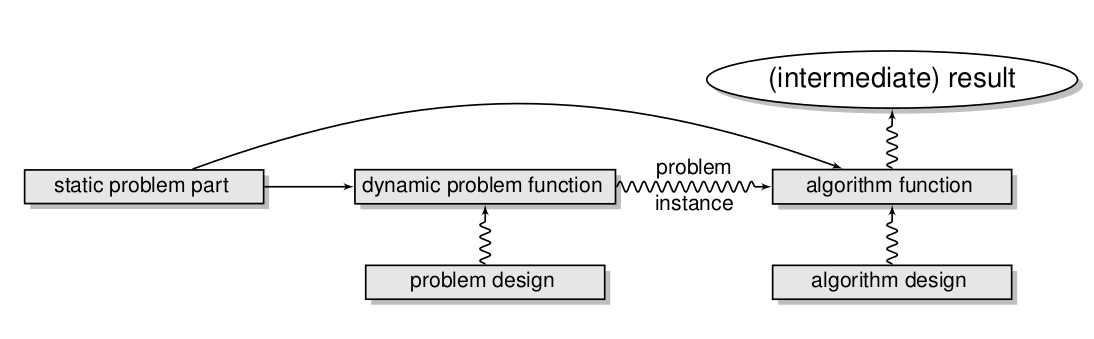
\includegraphics{figure/experiments.png}
  \begin{itemize}
    \item Problem definition split into static and dynamic part
      \begin{itemize}
        \item Immutable \texttt{R} objects: matrix, data frames, ...
        \item Arbitrary \texttt{R} function: transformations of static part, extraction of data from external sources, ...
      \end{itemize}
    \item Parametrization through specifying experimental designs for both problems and algorithms
    \item Each step automatically seeded, random seeds stored in a database
  \end{itemize}
\end{frame}

\begin{frame}[fragile]{Experiment definition steps}
  \begin{itemize}
    \item Add problems to registry: \texttt{addProblem}
      \begin{itemize}
        \item Efficient storage: Separation of static (\texttt{data}) and dynamic (\texttt{instance}) problem parts.
      \end{itemize}
    \item Add algorithms to registry: \texttt{addAlgorithm}
      \begin{itemize}
        \item Problem instance gets passed to algorithm
        \item Can be connected with an experimental design (function parameters)
        \item Return value will be saved on the file system
      \end{itemize}
    \item Add experiments to registry: \texttt{addExperiments}
      \begin{itemize}
        \item Experiment: problem instance + algorithm + algorithm parameters
        \item Job: Experiment + replication number
      \end{itemize}
  \end{itemize}
\end{frame}

\begin{frame}[fragile]{A simple Example}
  
\begin{lstlisting}
reg = makeExperimentRegistry("test_reg")
addProblem(name = "p1", data = 1, seed = 1,
  fun = function(data, job) runif(data))
addAlgorithm(name = "a1",
  fun = function(job, data, instance) 2 * instance)
addAlgorithm(name = "a2",
  fun = function(job, data, instance) data + instance)
addExperiments(repls = 2

)
submitJobs()
res = reduceResultsDataTable()
getJobPars()[res]

##    job.id problem prob.pars algorithm algo.pars result
## 1:      1      p1    <list>        a1    <list>  0.531
## 2:      2      p1    <list>        a1    <list>   0.37
## 3:      3      p1    <list>        a2    <list>   1.27
## 4:      4      p1    <list>        a2    <list>   1.18
\end{lstlisting}
  
\end{frame}

\begin{frame}[fragile]{Summary}
  \begin{itemize}
    \item Reproducibility: Every computation is seeded, seeds are stored in a \texttt{data.table}
    \item Portability: Data, algorithms, results and job information reside in a single directory
    \item Extensibility: Add more problems or algorithms, try different parameters or increase the replication numbers at any computational state
    \item Exchangeability: Share your file directory to allow others to extend your study with their data sets and algorithms
  \end{itemize}
  \begin{itemize}
    \item Greatly simplifies the work with batch systems
    \item Interactively control batch systems from within R (no shell required)
    \item Do reproducible research
    \item Exchange code and results with others
  \end{itemize}
\end{frame}

\endlecture
\end{document}
